\documentclass[10pt,openany,a4paper]{article}
\usepackage{amsmath, amsfonts, amssymb, amsthm}
\usepackage{tikz, pgfplots, tkz-euclide,calc}
    \usetikzlibrary{patterns,snakes,shapes.arrows}
\usepackage{fancyhdr}
\usepackage{enumerate,enumitem}
\usepackage{cancel}
\usepackage{varwidth}
\usepackage{hyperref}
\hypersetup{
    colorlinks=true,
    linkcolor=blue,
    filecolor=magenta,      
    urlcolor=cyan,
    }

% TAMBAHKAN PACKAGE SENDIRI KALAU KURANG

\usepackage{geometry}
\geometry{
	total = {160mm, 237mm},
	left = 25mm,
	right = 20mm,
	top = 30mm,
	bottom = 30mm,
}


\pagestyle{fancy}
\fancyhead{}
\fancyfoot{}
\fancyhead[r]{}
\fancyhead[l]{\fbox{\large{\textbf{SKPB - ITS}}}}
\renewcommand{\headrulewidth}{0pt}
\renewcommand{\footrulewidth}{0pt}
\renewcommand{\hrulefill}{\leavevmode\leaders\hrule height 2pt\hfill\kern0pt}

\begin{document}
    \begin{center}
	{\underline{\textbf{\MakeUppercase{Evaluasi Tengah Semester Bersama Gasal 2023/2024}}}}
    \end{center}

    \begin{center}
	\begin{tabular}{lcl}
		Mata kuliah/SKS & : & Kalkulus 1 ( SM234101 ) / 3 SKS\\
		Hari, Tanggal & : & Senin, 16 Oktober 2023\\
		Waktu & : & 07.00-08.40 WIB (100 menit)\\
		Sifat & : & Tertutup\\
		Kelas & : & 4-10
	\end{tabular}
    \end{center}
	
    \noindent\rule{\textwidth}{2.pt}
	
    \setlength{\parindent}{5pt}
    \par Diberikan 5 soal, dengan bobot nilai masing-masing soal sama dan boleh dikerjakan tidak berurutan.
    \setlength{\parindent}{5pt}
    \centering{Tuliskan: Nama, NRP, dan Nomor Kelas pada lembar jawaban Anda.}
    \setlength{\parindent}{5pt}
    {\small
    \par \textbf{\MakeUppercase{Dilarang membawa/menggunakan kalkulator dan alat komunikasi}}
    \centering{\textbf{\MakeUppercase{dilarang memberikan/menerima jawaban selama ujian}}}}
    \par \centering{\textbf{"Setiap tindak kecurangan akan mendapat sanksi akademik."}}
	
    \noindent\rule{\textwidth}{2.pt}
	
% SOAL DI SINI YAA
    \begin{enumerate}
        \item Diberikan tiga titik koordinat \( A(-1,3) \), \( B(1,-2) \), dan \( C(3,0) \).
        \begin{enumerate}
            \item Dapatkan persamaan garis lurus \( g \) yang melalui titik \( B \) dan \( C \).
            \item Dapatkan persamaan garis lurus \( k \) yang melalui titik \( A \) dan tegak lurus dengan garis \( g \).
            \item Dapatkan jarak titik \( A \) ke garis lurus \( g \).
        \end{enumerate}
        
        \item Diketahui \( f(x) = \dfrac{4}{x^2 - 1} \) dan \( g(x) = \sqrt{x+4} \).
        \begin{enumerate}
            \item Dapatkan domain \( f \) dan \( g \).
            \item Dapatkan \( (g \circ f)(x) \) beserta domainnya.
        \end{enumerate}
        
        \item Diberikan fungsi \( f(x) = 1 + \sqrt{8 - x^2} \).
        \begin{enumerate}
            \item Dapatkan invers fungsi \( f(x) \).
            \item Dapatkan domain dan range invers fungsinya.
        \end{enumerate}
        
        \item Diberikan $f(x) =\begin{cases}2k^2(x - 1), & x \leq 2 \\
            \,\\
            \left(\dfrac{1 - k}{2}\right)x, & x > 2\end{cases}$\\
        Tentukan semua nilai \( k \) yang memenuhi agar \( \lim\limits_{x \to 2} f(x) \) ada.
        
        \item Gunakan diferensiasi implisit untuk mendapatkan \( \dfrac{dy}{dx} \) dari persamaan $y - x^2 y^3 = y^2 x - x.$
    \end{enumerate}
	
    \fancyfoot{
    \hrulefill\textbf{ Selamat Mengerjakan }\hrulefill

    \begin{center}
	    ``\textit{Jujur adalah kunci kesuksesan}''
    \end{center}}

    \newpage
    \fancyhead[L]{\textit{Solution By: \hyperlink{https://github.com/TetewHeroez}{Tetew}}}
    % \fancyfoot[R]{\animategraphics[autoplay,loop,width=0.1\textwidth]{15}{Kuru Kuru Herta/kuru kuru-}{0}{5}}
    \fancyfoot{}
    {\centering\textbf{SOLUSI}}
    \renewcommand{\headrulewidth}{1pt}
    \begin{enumerate}
        \item 
    \end{enumerate}
    \newpage
    \fancyhead{}
    \fancyhead[r]{}
    \fancyhead[l]{\fbox{\large{\textbf{SKPB - ITS}}}}
    \renewcommand{\headrulewidth}{0pt}

    \begin{center}
	{\underline{\textbf{\MakeUppercase{Evaluasi Tengah Semester Bersama Gasal 2023/2024}}}}
    \end{center}

    \begin{center}
	\begin{tabular}{lcl}
		Mata kuliah/SKS & : & Kalkulus 1 ( SM234101 ) / 3 SKS\\
		Hari, Tanggal & : & Senin, 16 Oktober 2023\\
		Waktu & : & 09.00-10.40 WIB (100 menit)\\
		Sifat & : & Tertutup\\
		Kelas & : & 11-16
	\end{tabular}
    \end{center}
	
    \noindent\rule{\textwidth}{2.pt}
	
    \setlength{\parindent}{5pt}
    \par Diberikan 5 soal, dengan bobot nilai masing-masing soal sama dan boleh dikerjakan tidak berurutan.
    \setlength{\parindent}{5pt}
    \centering{Tuliskan: Nama, NRP, dan Nomor Kelas pada lembar jawaban Anda.}
    \setlength{\parindent}{5pt}
    {\small
    \par \textbf{\MakeUppercase{Dilarang membawa/menggunakan kalkulator dan alat komunikasi}}
    \centering{\textbf{\MakeUppercase{dilarang memberikan/menerima jawaban selama ujian}}}}
    \par \centering{\textbf{"Setiap tindak kecurangan akan mendapat sanksi akademik."}}
	
    \noindent\rule{\textwidth}{2.pt}
	
% SOAL DI SINI YAA
\begin{enumerate}
    \item Dapatkan himpunan penyelesaian dari pertidaksamaan
    \[
    \frac{\frac{1}{3}x - 5}{2x - 5} \geq 3
    \]

    \item Diberikan $f(x) = x^2 - 1$ dan $g(x) = \sqrt{x - 3}$.
    \begin{enumerate}
        \item Dapatkan domain $f$ dan $g$
        \item Dapatkan $(g \circ f)(x)$ beserta domainnya.
    \end{enumerate}

    \item Diberikan fungsi $f(x) = x^2 - 4x + 5$.
    \begin{enumerate}
        \item Tentukan nilai $k$ terkecil sehingga $f(x)$ memiliki invers pada $[k, \infty)$
        \item Tentukan invers fungsi $f(x)$.
    \end{enumerate}

    \item Diketahui $f(x) = \dfrac{1}{|3 - x|}$
    \begin{enumerate}
        \item Hitunglah $\displaystyle\lim_{x \to 3} f(x)$.
        \item Berapa nilai $f(3)$?
        \item Apakah $f(x)$ kontinu? Jelaskan!
        \item Apakah diskontinuitas $f(x)$ dapat dihilangkan? jika iya, definisikan kembali $f(x)$ sehingga menjadi kontinu.
    \end{enumerate}

    \item Gunakan diferensiasi implisit untuk mendapatkan $\dfrac{dy}{dx}$ dari $x^3 y^3 - 2y^2 - 3x + 7 = 0.$
\end{enumerate}
	
    \fancyfoot{
    \hrulefill\textbf{ Selamat Mengerjakan }\hrulefill

    \begin{center}
	    ``\textit{Jujur adalah kunci kesuksesan}''
    \end{center}}

    \newpage
    \fancyhead[L]{\textit{Solution By: \hyperlink{https://github.com/TetewHeroez}{Tetew}}}
    % \fancyfoot[R]{\animategraphics[autoplay,loop,width=0.1\textwidth]{15}{Kuru Kuru Herta/kuru kuru-}{0}{5}}
    \fancyfoot{}
    {\centering\textbf{SOLUSI}}
    \renewcommand{\headrulewidth}{1pt}
    \begin{enumerate}
        \item .
        \item .
        \item .
        \item 
    \end{enumerate}

    \newpage
    \fancyhead{}
    \fancyhead[r]{}
    \fancyhead[l]{\fbox{\large{\textbf{SKPB - ITS}}}}
    \renewcommand{\headrulewidth}{0pt}
    
    \begin{center}
	{\underline{\textbf{\MakeUppercase{Evaluasi Tengah Semester Bersama Gasal 2023/2024}}}}
    \end{center}

    \begin{center}
	\begin{tabular}{lcl}
		Mata kuliah/SKS & : & Kalkulus 1 ( SM234101 ) / 3 SKS\\
		Hari, Tanggal & : & Senin, 16 Oktober 2023\\
		Waktu & : & 11.00-12.40 WIB (100 menit)\\
		Sifat & : & Tertutup\\
		Kelas & : & 31-37
	\end{tabular}
    \end{center}
	
    \noindent\rule{\textwidth}{2.pt}
	
    \setlength{\parindent}{5pt}
    \par Diberikan 5 soal, dengan bobot nilai masing-masing soal sama dan boleh dikerjakan tidak berurutan.
    \setlength{\parindent}{5pt}
    \centering{Tuliskan: Nama, NRP, dan Nomor Kelas pada lembar jawaban Anda.}
    \setlength{\parindent}{5pt}
    {\small
    \par \textbf{\MakeUppercase{Dilarang membawa/menggunakan kalkulator dan alat komunikasi}}
    \centering{\textbf{\MakeUppercase{dilarang memberikan/menerima jawaban selama ujian}}}}
    \par \centering{\textbf{"Setiap tindak kecurangan akan mendapat sanksi akademik."}}
	
    \noindent\rule{\textwidth}{2.pt}
	
% SOAL DI SINI YAA
\begin{enumerate}
    \item Dapatkan himpunan penyelesaian dari pertidaksamaan
    \[
    \frac{x - 1}{2 - x} \geq \frac{x + 1}{x + 2}
    \]

    \item Diketahui $f(x) = \sqrt{x + 1}$ dan $g(x) = \sqrt{4 - x^2}$.
    \begin{enumerate}
        \item Dapatkan domain $f$ dan $g$
        \item Dapatkan $(g \circ f)(x)$ beserta domainnya.
    \end{enumerate}

    \item Diberikan suatu fungsi $f(x) = 2 + \sqrt{4 - x}$ dengan domain $f$ adalah $[a,2]$.
    \begin{enumerate}
        \item Tentukan nilai terkecil $a$ agar $f^{-1}(x)$ ada.
        \item Dapatkan $f^{-1}(x)$
        \item Sketsa grafik $f(x)$ dan $f^{-1}(x)$ pada satu bidang koordinat.
    \end{enumerate}

    \item Diberikan $f(x) = \begin{cases}\dfrac{x^3 - 2x^2 + x - 1}{x - 1}, & x \neq 1 \\k, & x = 1\end{cases}$
    Tentukan nilai $k$, sehingga $f(x)$ kontinu.

    \item Dapatkan persamaan garis singgung kurva $x^3 y + 4xy = 12y$ di titik $(2,1)$.
\end{enumerate}
	
    \fancyfoot{
    \hrulefill\textbf{ Selamat Mengerjakan }\hrulefill

    \begin{center}
	    ``\textit{Jujur adalah kunci kesuksesan}''
    \end{center}}

    \newpage
    \fancyhead[L]{\textit{Solution By: \hyperlink{https://github.com/TetewHeroez}{Tetew}}}
    % \fancyfoot[R]{\animategraphics[autoplay,loop,width=0.1\textwidth]{15}{Kuru Kuru Herta/kuru kuru-}{0}{5}}
    \fancyfoot{}
    {\centering\textbf{SOLUSI}}
    \renewcommand{\headrulewidth}{1pt}
    \begin{enumerate}
        \item 
    \end{enumerate}

    \newpage
    \fancyhead{}
    \fancyhead[r]{}
    \fancyhead[l]{\fbox{\large{\textbf{SKPB - ITS}}}}
    \renewcommand{\headrulewidth}{0pt}
    
    \begin{center}
	{\underline{\textbf{\MakeUppercase{Evaluasi Tengah Semester Bersama Gasal 2023/2024}}}}
    \end{center}

    \begin{center}
	\begin{tabular}{lcl}
		Mata kuliah/SKS & : & Kalkulus 1 ( SM234101 ) / 3 SKS\\
		Hari, Tanggal & : & Selasa, 17 Oktober 2023\\
		Waktu & : & 07.00-08.40 WIB (100 menit)\\
		Sifat & : & Tertutup\\
		Kelas & : & 17-23
	\end{tabular}
    \end{center}
	
    \noindent\rule{\textwidth}{2.pt}
	
    \setlength{\parindent}{5pt}
    \par Diberikan 5 soal, dengan bobot nilai masing-masing soal sama dan boleh dikerjakan tidak berurutan.
    \setlength{\parindent}{5pt}
    \centering{Tuliskan: Nama, NRP, dan Nomor Kelas pada lembar jawaban Anda.}
    \setlength{\parindent}{5pt}
    {\small
    \par \textbf{\MakeUppercase{Dilarang membawa/menggunakan kalkulator dan alat komunikasi}}
    \centering{\textbf{\MakeUppercase{dilarang memberikan/menerima jawaban selama ujian}}}}
    \par \centering{\textbf{"Setiap tindak kecurangan akan mendapat sanksi akademik."}}
	
    \noindent\rule{\textwidth}{2.pt}
	
% SOAL DI SINI YAA
\begin{enumerate}
    \item Dapatkan himpunan penyelesaian pertidaksamaan
    \[
    2 \leq \frac{x^2 + 1}{x} < x + 3
    \]

    \item Diberikan fungsi $f(x) = \sqrt{5 - x}$ dan $g(x) = \dfrac{1}{9 - x^2}$.
    \begin{enumerate}
        \item Dapatkan domain $f$ dan $g$
        \item Dapatkan $(g \circ f)(x)$ beserta domainnya.
    \end{enumerate}

    \item Diketahui $f(x) = \sqrt{4 - x^2}$.
    \begin{enumerate}
        \item Tentukan domain $f(x)$.
        \item Apakah $f^{-1}(x)$ ada? Jelaskan alasannya.
        \item Jika tidak ada, definisikan domain $f(x)$ agar $f^{-1}(x)$ ada.
    \end{enumerate}

    \item Hitunglah $\displaystyle\lim_{x \to 3} \frac{\sqrt{x^2 - 5} - 2}{x - 3}$

    \item Diberikan $f(x) = \dfrac{x + 3}{x + 2}$
    \begin{enumerate}
        \item Dapatkan $\dfrac{dy}{dx}$.
        \item Jika $(x_0, y_0)$ merupakan titik pada kurva $f(x)$, maka dapatkan titik $(x_0, y_0)$ dan garis singgung di $(x_0, y_0)$ yang tegak lurus dengan $y = x$.
    \end{enumerate}
\end{enumerate}
	
    \fancyfoot{
    \hrulefill\textbf{ Selamat Mengerjakan }\hrulefill

    \begin{center}
	    ``\textit{Jujur adalah kunci kesuksesan}''
    \end{center}}

    \newpage
    \fancyhead[L]{\textit{Solution By: \hyperlink{https://github.com/TetewHeroez}{Tetew}}}
    % \fancyfoot[R]{\animategraphics[autoplay,loop,width=0.1\textwidth]{15}{Kuru Kuru Herta/kuru kuru-}{0}{5}}
    \fancyfoot{}
    {\centering\textbf{SOLUSI}}
    \renewcommand{\headrulewidth}{1pt}
    \begin{enumerate}
        \item 
    \end{enumerate}

    \newpage

    \fancyhead{}
    \fancyhead[r]{}
    \fancyhead[l]{\fbox{\large{\textbf{SKPB - ITS}}}}
    \renewcommand{\headrulewidth}{0pt}

    \begin{center}
	{\underline{\textbf{\MakeUppercase{Evaluasi Tengah Semester Bersama Genap 2023/2024}}}}
    \end{center}

    \begin{center}
	\begin{tabular}{lcl}
		Mata kuliah/SKS & : & Kalkulus 1 ( SM234101 ) / 3 SKS\\
		Hari, Tanggal & : & Selasa, 17 Oktober 2023\\
		Waktu & : & 09.00-10.40 WIB (100 menit)\\
		Sifat & : & Tertutup\\
		Kelas & : & 24-30
	\end{tabular}
    \end{center}
	
    \noindent\rule{\textwidth}{2.pt}
	
    \setlength{\parindent}{5pt}
    \par Diberikan 5 soal, dengan bobot nilai masing-masing soal sama dan boleh dikerjakan tidak berurutan.
    \setlength{\parindent}{5pt}
    \centering{Tuliskan: Nama, NRP, dan Nomor Kelas pada lembar jawaban Anda.}
    \setlength{\parindent}{5pt}
    {\small
    \par \textbf{\MakeUppercase{Dilarang membawa/menggunakan kalkulator dan alat komunikasi}}
    \centering{\textbf{\MakeUppercase{dilarang memberikan/menerima jawaban selama ujian}}}}
    \par \centering{\textbf{"Setiap tindak kecurangan akan mendapat sanksi akademik."}}
	
    \noindent\rule{\textwidth}{2.pt}
	
% SOAL DI SINI YAA
    \begin{enumerate}
	\item Tentukan semua nilai $x$ yang memenuhi
        \[1<\frac{1}{|x-2|}\leq4\]

        \item diketahui $f(x)=\dfrac{1+x}{1-x}$ dan $g(x)=\dfrac{x}{1-x}$,
        \begin{enumerate}
            \item Dapatkan domain $f$ dan $g$.
            \item Dapatkan $(f\circ g)(x)$ beserta domainnya.
        \end{enumerate}

        \item Diberikan fungsi $f(x)=x^2-2x+1$
        \begin{enumerate}
            \item Tentukan nilai $k$ terbesar sehingga $f(x)$ memiliki invers pada $[-\infty,k]$.
            \item Tentukan $f^{-1}(x)$.
            \item Sketsa grafik $f(x)$ dan $f^{-1}(x)$ dalam satu bidang koordinat.
        \end{enumerate}

        \item Diberikan fungsi $f(x)=\begin{cases}
        2|x+1|&   x < -1\\
        \\
        x^2 &   x \geq 1
        \end{cases}$
        \begin{enumerate}
            \item hitunglah $\lim\limits_{x\to-1}f(x)$.
            \item Berapa nilai $f(-1)$?
            \item Apakah $f(x)$ kontinu? jelaskan!
        \end{enumerate}
        Apakah $f(x)$ kontinu di $x=-1$? jelaskan!

        \item Diketahui garis singgung pada kurva $y^3=2x^2$ di titik $(a,b)$ sejajar dengan garis $2x+3y-5=0$. Tentukan titik $(a,b)$.
    \end{enumerate}
	
    \fancyfoot{
    \hrulefill\textbf{ Selamat Mengerjakan }\hrulefill

    \begin{center}
	    ``\textit{Jujur adalah kunci kesuksesan}''
    \end{center}}

    \newpage
    \fancyhead[L]{\textit{Solution By: \hyperlink{https://github.com/TetewHeroez}{Tetew}}}
    % \fancyfoot[R]{\animategraphics[autoplay,loop,width=0.1\textwidth]{15}{Kuru Kuru Herta/kuru kuru-}{0}{5}}
    \fancyfoot{}
    {\centering\textbf{SOLUSI}}
    \renewcommand{\headrulewidth}{1pt}
    \begin{enumerate}
        \item Bagi kasus pada pertidaksamaan.
        \begin{enumerate}[label=(\arabic*)]
            \item Untuk $1<\frac{1}{|x-2|}$ diperoleh:\\
            \textit{(*Catatan: Hasil nilai mutlak selalu positif, sehingga jika kedua ruas dikali $|x-2|$ tidak akan mengubah tanda pertidaksamaan)}
            \begin{align*}
                1<\frac{1}{|x-2|}&\hspace{4.0cm}\\
                1|x-2|<1&,\quad x\neq2 \textrm{\textbf{ (Penyebut tak nol)}}\\
                |x-2|<1&,\quad x\neq2\\
                -1<x-2<1&,\quad x\neq2 \textrm{\textbf{ (Definisi jarak)}}\\
                1<x<3&,\quad x\neq2\\
            \end{align*}
            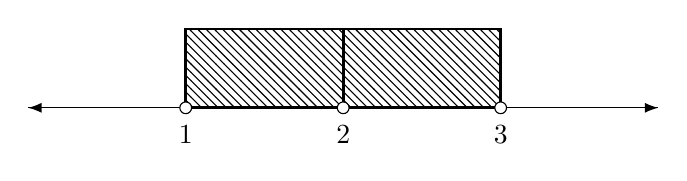
\begin{tikzpicture}
                \draw[-Latex] (0,0) -- (8,0);
                \draw[Latex-] (0,0) -- (8,0);
                \foreach \i in {1,2,3}
                {
                \coordinate (A\i) at ({2*\i},0);
                \node[below] at ($(0,-0.1)+(A\i)$) {$\i$};
                }
                
                \draw[fill=lightgray,pattern=north west lines,line width=1pt](A1)rectangle($(A2)+(0,1)$);
                \draw[fill=lightgray,pattern=north west lines,line width=1pt](A2)rectangle($(A3)+(0,1)$);
                
                \foreach \i in {1,2,3}
                \node[circle,draw,fill=white,inner sep=1.5pt] at (A\i) {};
                
            \end{tikzpicture}\\
            $HP_1=\{x\:|\:1<x<2 \:\vee\: 2<x<3\}=(1,2)\cup(2,3)$

            \item Untuk $\frac{1}{|x-2|}\leq4$ diperoleh:\\
            \begin{align*}
                \frac{1}{|x-2|}\leq4&\hspace{4.0cm}\\
                1\leq4|x-2|&,\quad x\neq2 \textrm{\textbf{ (Penyebut tak nol)}}\\
                \frac{1}{4}\leq|x-2|&,\quad x\neq2\\
                \frac{1}{4}\leq x-2\:\bigvee\:-\frac{1}{4}\geq x-2&,\quad x\neq2 \textrm{\textbf{ (Definisi jarak)}}\\
                \frac{1}{4}+2\leq x\:\bigvee\:-\frac{1}{4}+2\geq x&,\quad x\neq2\\
                \frac{9}{4}\leq x\:\bigvee\:\frac{7}{4}\geq x&,\quad x\neq2
            \end{align*}
            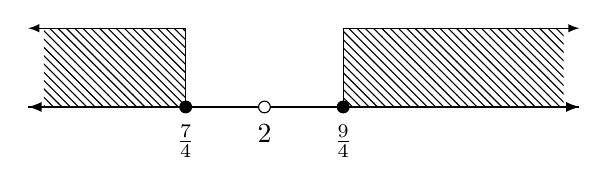
\begin{tikzpicture}
                \draw[-Latex] (-1,0) -- (6,0);
                \draw[Latex-] (-1,0) -- (6,0);
                \foreach \i in {1,2,3}
                \coordinate (A\i) at (\i,0);
                \node[below] at ($(0,-0.1)+(A1)$) {$\frac{7}{4}$};
                \node[below] at ($(0,-0.1)+(A2)$) {$2$};
                \node[below] at ($(0,-0.1)+(A3)$) {$\frac{9}{4}$};

                \fill[lightgray,pattern=north west lines,line width=1pt](A1)rectangle($(-0.8,0)+(0,1)$);
                \fill[lightgray,pattern=north west lines,line width=1pt](A3)rectangle($(5.8,0)+(0,1)$);
                
                \draw[-latex](A1)--($(A1)+(0,1)$)--($(-1,0)+(0,1)$);
                \draw[-latex](A3)--($(A3)+(0,1)$)--($(6,0)+(0,1)$);
                
                \foreach \i in {1,3}
                \node[circle,draw,fill=black,inner sep=1.5pt] at (A\i) {};
                \node[circle,draw,fill=white,inner sep=1.5pt] at (A2) {};
                
            \end{tikzpicture}\\
            $HP_2=\left\{x\:|\:x\leq\frac{7}{4} \:\vee\: x\geq\frac{9}{4}\right\}=\left(-\infty,\frac{7}{4}\right]\cup\left[\frac{9}{4},+\infty\right)$
        \end{enumerate}
        Sehingga irisan kedua himpunan penyelasaian\\~\\
        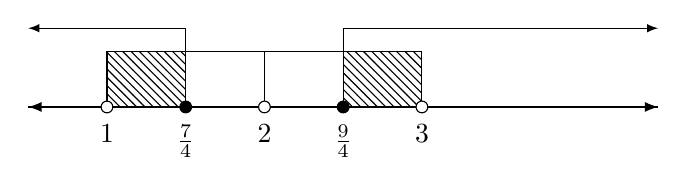
\begin{tikzpicture}
            \draw[-Latex] (0,0) -- (8,0);
            \draw[Latex-] (0,0) -- (8,0);
            \foreach \i in {1,2,3,4,5}
                \coordinate (A\i) at (\i,0);
            \node[below] at ($(0,-0.1)+(A1)$) {$1$};
            \node[below] at ($(0,-0.1)+(A2)$) {$\frac{7}{4}$};
            \node[below] at ($(0,-0.1)+(A3)$) {$2$};
            \node[below] at ($(0,-0.1)+(A4)$) {$\frac{9}{4}$};
            \node[below] at ($(0,-0.1)+(A5)$) {$3$};

            \fill[lightgray,pattern=north west lines,line width=1pt](A1)rectangle($(A2)+(0,0.7)$);
             \fill[lightgray,pattern=north west lines,line width=1pt](A4)rectangle($(A5)+(0,0.7)$);

            \draw(A1)rectangle($(A3)+(0,0.7)$);
            \draw(A3)rectangle($(A5)+(0,0.7)$);
            \draw[-latex](A2)--($(A2)+(0,1)$)--($(0,0)+(0,1)$);
            \draw[-latex](A4)--($(A4)+(0,1)$)--($(8,0)+(0,1)$);

            \foreach \i in {1,3,5}
                \node[circle,draw,fill=white,inner sep=1.5pt] at (A\i) {};
            \foreach \i in {2,4}
                 \node[circle,draw,fill=black,inner sep=1.5pt] at (A\i) {};
        \end{tikzpicture}\\
        $HP=HP_1\cap HP_2=\left\{x\:|\:1<x\leq\frac{7}{4}\:\vee\:\frac{9}{4}\leq x<3\right\}=\left(1,\frac{7}{4}\right]\cup\left[\frac{9}{4},3\right)$.
        
        \item \begin{enumerate}
            \item Karena fungsi berbentuk pecahan, maka penyebutnya tidak boleh nol.
            \begin{flalign*}
                D_f&=\{x\:|\:x\neq 1\}&\\
                D_g&=\{x\:|\:x\neq 1\}
            \end{flalign*}

            \item Ingat bahwa $(f\circ g)(x)=f(g(x))$, sehingga
            \begin{flalign*}
                f(g(x))&=\frac{1+g(x)}{1-g(x)}&\\
                &=\frac{1+(\frac{x}{1-x})}{1-(\frac{x}{1-x})}\quad\quad\textrm{\textbf{$\left(\textrm{Subtitusi }g(x)=\frac{x}{1-x}\right)$}}&\\
                &=\frac{(\frac{1-x+x}{1-x})}{(\frac{1-x-x}{1-x})}&\\
                &=\frac{\frac{1-x+x}{\cancel{1-x}}}{\frac{1-x-x}{\cancel{1-x}}},\quad x\neq1&\\
                &=\frac{1}{1-2x},\quad x\neq1
            \end{flalign*}
            Definisi domain fungsi komposisi $f\circ g$ adalah $D_{f\circ g}=\{x\in D_g\:|\:g(x)\in D_f\}$.
            \begin{flalign*}
                D_{f\circ g}&=\{x\in \mathbb{R}/\{1\}\:|\:g(x)\in \mathbb{R}/\{1\}\}&\\
                &=\left\{x\in \mathbb{R}/\{1\}\:\Big|\:\underbrace{\frac{x}{1-x}\in \mathbb{R}/\{1\}}\right\}&\\
                &\fbox{$\displaystyle\frac{x}{1-x}\neq1$}\Rightarrow \fbox{$\displaystyle x\neq1-x$}\Rightarrow \fbox{$\displaystyle2x\neq1$}\Rightarrow \fbox{$\displaystyle x\neq\frac{1}{2}$}&\\
                &=\left\{x\in \mathbb{R}/\{1\}\:\Big|\:x\in \mathbb{R}\Big/\left\{\frac{1}{2}\right\}\right\}&\\
                &=\left\{x\in \mathbb{R}\Big/\left\{1,\frac{1}{2}\right\}\right\}&\\
            \end{flalign*}
            $\therefore(f\circ g)(x)=\frac{1}{1-2x}$ dan $D_{f\circ g}=\{x\:|\:x\neq1\:\vee\:x\neq\frac{1}{2}\}$
        \end{enumerate}

        \item \begin{enumerate}
            \item Perhatikan bahwa $f(x)=x^2-2x+1=(x-1)^2$. agar $f(x)$ mempunyai invers maka haruslah $f(x)$ fungsi satu-satu. Gambar grafiknya sebagai berikut:\\
            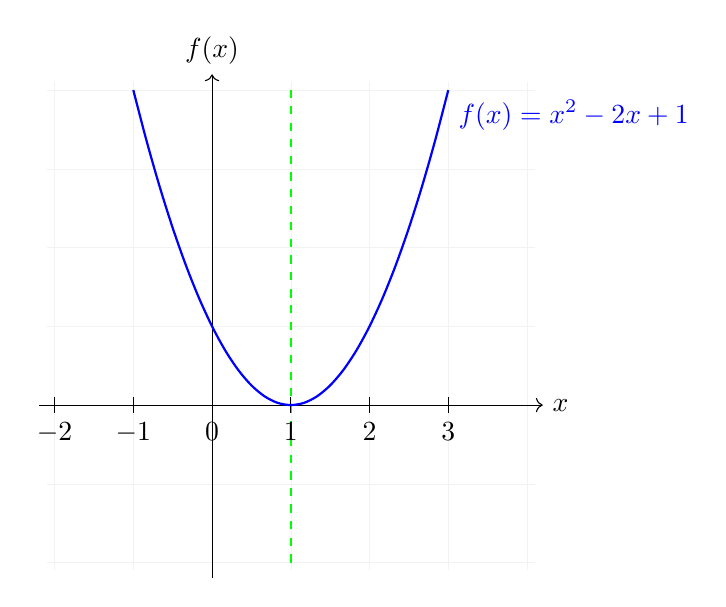
\begin{tikzpicture}
                \draw[very thin,color=lightgray!20] (-2.1,-2.1) grid (4.1,4.1);
                \draw[->] (-2.2,0) -- (4.2,0) node[right] {$x$};
                \draw[->] (0,-2.2) -- (0,4.2) node[above] {$f(x)$};
                
                \draw[thick,green,dashed,domain=-2:4,smooth]plot (1,\x);
                
                \foreach \x in {-2,-1,0,1,2,3} \draw[shift={(\x,0)},color=black] (0pt,3pt) -- (0pt,-3pt) node[below] {$\x$};
                
                \draw[thick,blue,domain=-1:3,smooth] plot (\x,{(\x-1)^2}) node [below right] {$f(x)=x^2-2x+1$};
            \end{tikzpicture}\\
            Perhatikan bahwa $f(x)$ simetri terhadap garis $x=1$. Ketika ingin mengambil $k$ terbesar agar $f(x)$ punya invers, haruslah pilih $k=1$ sehingga interval domainnya menjadi $[-\infty,1]$.\\~\\
            \textit{(*Catatan: Secara geometris suatu fungsi dikatakan punya invers ketika kita menggambar sebarang garis horizontal yang melewati grafik fungsi tersebut sedemikian sehingga hanya terdapat maksimal satu titik potong antara garis horizontal dan grafik fungsi tersebut. lebih jelasnya perhatikan gambar berikut)}\\
            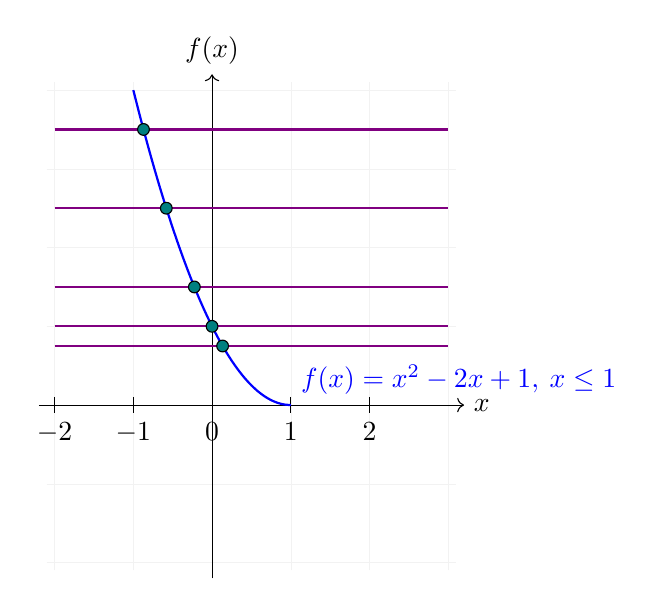
\begin{tikzpicture}
                \draw[very thin,color=lightgray!20] (-2.1,-2.1) grid (3.1,4.1);
                \draw[->] (-2.2,0) -- (3.2,0) node[right] {$x$};
                \draw[->] (0,-2.2) -- (0,4.2) node[above] {$f(x)$};
                
                \foreach \x in {-2,-1,0,1,2} \draw[shift={(\x,0)},color=black] (0pt,3pt) -- (0pt,-3pt) node[below] {$\x$};
                
                \draw[thick,blue,domain=-1:1,smooth] plot (\x,{(\x-1)^2}) node [above right] {$f(x)=x^2-2x+1,\:x\leq1$};

                \foreach \y in {3,2,1,0.5,0.25}
                {
                \draw[thick,violet,domain=-2:3,smooth]plot ({\x},{\y+0.5});
                \node[circle,draw,fill=teal,inner sep=1.5pt] at ({-sqrt(\y+0.5)+1},{\y+0.5}) {};
                }
            \end{tikzpicture}\\
            
            \item Gantikan $y$ dengan $x$ dan juga sebaliknya.
            \begin{flalign*}
                x&=(y-1)^2&\\
                x&=(y-1)^2&\\
                \sqrt{x}&=\sqrt{y-1)^2}&\\
                \sqrt{x}&=|y-1|&\\
                \pm\sqrt{x}&=y-1&\\
                y&=1\pm\sqrt{x}&\\
                f^{-1}(x)&=1\pm\sqrt{x}&\\
            \end{flalign*}
            
            Karena range $R_{f^{-1}}=D_f=[-\infty,1]$, maka $f^{-1}(x)=1-\sqrt{x}$.\\~\\

            \item Salah satu cara menggambar grafik $f^{-1}(x)$ adalah dengan mencerminkan $f(x)$ terhadap garis $y=x$, sehingga akan didapat grafik $f^{-1}(x)$.\\
            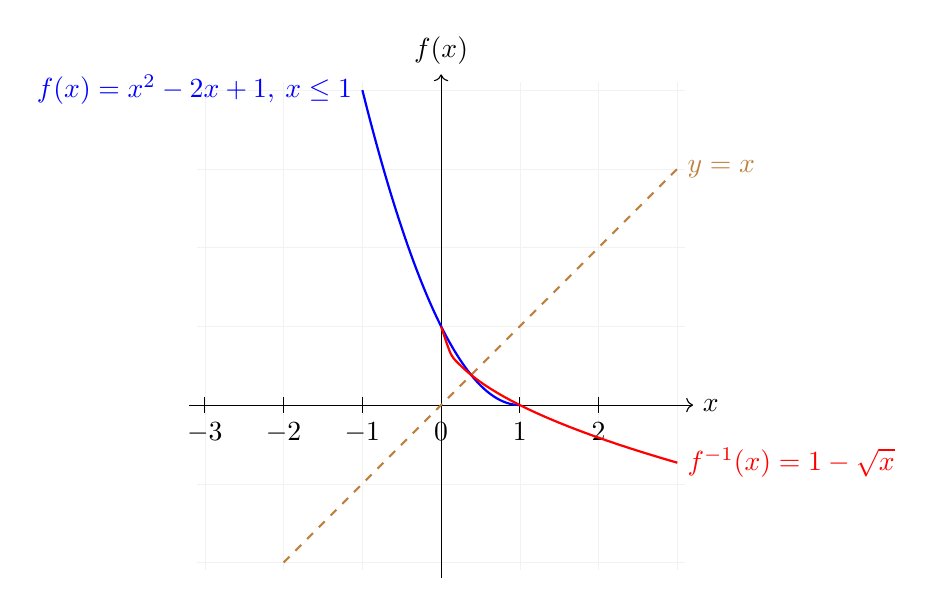
\begin{tikzpicture}
                \draw[very thin,color=lightgray!20] (-3.1,-2.1) grid (3.1,4.1);
                \draw[->] (-3.2,0) -- (3.2,0) node[right] {$x$};
                \draw[->] (0,-2.2) -- (0,4.2) node[above] {$f(x)$};
                
                \foreach \x in {-3,-2,-1,0,1,2} \draw[shift={(\x,0)},color=black] (0pt,3pt) -- (0pt,-3pt) node[below] {$\x$};

                \draw[thick,brown,dashed,domain=-2:3,smooth] plot (\x,\x) node [right] {$y=x$};
                \draw[thick,blue,domain=1:-1,smooth] plot (\x,{(\x-1)^2}) node [left] {$f(x)=x^2-2x+1,\:x\leq1$};
                \draw[thick,red,domain=0:3,smooth] plot (\x,{1-sqrt(\x)}) node [right] {$f^{-1}(x)=1-\sqrt{x}$};

            \end{tikzpicture}\\
            \end{enumerate}
            
            \item Secara definisi $f(x)=\begin{cases}
        2|x+1|&   x < -1\begin{cases}
            2x+2&\quad x>=-1,x<-1\\
             -2x-2&\quad x<-1,x<-1
        \end{cases}\\
        \\
        x^2 &   x \geq -1
        \end{cases}$\\
        Perhatikan bahwa $(-\infty,-1)\cap[-1,+\infty)=\varnothing$, sehingga\\
        $f(x)=\begin{cases}
        2|x+1|&   x < -1\begin{cases}
            2x+2&\quad \varnothing\\
             -2x-2&\quad x<-1
        \end{cases}\\
        \\
        x^2 &   x \geq ‐1
        \end{cases}$\\~\\
        Dan dapat disederhanakan menjadi\\
        
        $f(x)=\begin{cases}
        -2x-2&   x < -1\\
        \\
        x^2 &   x \geq -1
        \end{cases}$
        \begin{enumerate}
            \item $\lim\limits_{x\to-1}f(x)=\begin{cases}
                    \lim\limits_{x\to-1^-}f(x)=\lim\limits_{x\to-1^-}-2x-2=0\\
                    \lim\limits_{x\to-1^+}f(x)=\lim\limits_{x\to-1^-}x^2=1
                \end{cases}$\\~\\
                Karena $\lim\limits_{x\to-1^-}f(x)\neq\lim\limits_{x\to-1^+}f(x)$, maka $\lim\limits_{x\to-1}f(x)$ tidak ada.\\

            \item $f(-1)=(-1)^2=1$\\
            
            \item $f(x)$ kontinu di titik $x=a$, jika memenuhi ketiga syarat:
            \begin{itemize}
                \item $f(a)$ terdefinisi.
                \item $\lim\limits_{x\to a}f(x)$ ada.
                \item $f(a)=\lim\limits_{x\to a}f(x)$
            \end{itemize}
            $f(x)$ tidak kontinu dimana-mana karena ada titik dimana $f(x)$ tidak kontinu, yaitu di $x=-1$. 
        \end{enumerate}
        $f(x)$ tidak kontinu di $x=-1$, karena pada soal (a) sudah disebutkan bahwa $\lim\limits_{x\to-1}f(x)$ tidak ada. Hal tersebut mengakibatkan syarat kedua dari $f(x)$ kontinu tidak terpenuhi.\\~\\
        
        \item Ingat bahwa $m_s=\frac{dy}{dx}$ dengan $m_s$ adalah garis singgung fungsi $y=f(x)$. Dengan turunan implisit akan didapatkan:
        \begin{flalign*}
            \frac{d}{dx}(y^3)&=\frac{d}{dx}(2x^2)&\\
            3y^2\frac{dy}{dx}&=4x&\\
            m_s&=\frac{dy}{dx}=\frac{4x}{3y^2},\quad y\neq0
        \end{flalign*}
        Karena garis singgung melewati $(a,b)$, maka $m_s=\frac{dy}{dx}\Big|_{\tiny{\begin{matrix}x=a\\y=b\end{matrix}}}=\frac{4a}{3b^2}$. Diketahui bahwa garis singgung sejajar dengan garis $l:=2x+3y-5=0$.
        \begin{flalign*}
            2x&+3y-5=0&\\
            3y&=-2x+5&\\
            y&=\underbrace{-\frac{2}{3}}_{m_l}x+\underbrace{\frac{5}{3}}_{c}\quad \left(\textrm{Bentuk \fbox{$y=m_lx+c$}}\right)
        \end{flalign*}
        Karena garis saling sejajar, maka
        \begin{flalign*}
            m_s&=m_l&\\
            \frac{4a}{\cancel{3}b^2}&=-\frac{2}{\cancel{3}}&\\
            4a&=-2b^2&\\
            a&=-\frac{1}{2}b^2...........(1)
        \end{flalign*}
        Ingat bahwa titik $(a,b)$ juga terletak pada $y^3=2x^2$, sehingga
        \begin{flalign*}
            (b)^3&=2(a)^2&\\
            b^3&=2a^2...........(2)
        \end{flalign*}
        Subtitusi persamaan $(1)$ ke persamaan $(2)$.
        \begin{flalign*}
            b^3&=2(-\frac{1}{2}b^2)^2&\\
            b^3&=\frac{1}{2}b^4&\\
            b^3-\frac{1}{2}b^4&=0&\\
            b^3(1-\frac{1}{2}b)&=0
        \end{flalign*}
        Didapatkan $b=0\:\vee\:b=2$. Subtitusi hasil tersebut ke persamaan $(1)$ atau $(2)$, sehingga didapat titik $(a,b)$ adalah $(0,0)$ dan $(-2,2)$. Namun karena $y\neq0$ maka satu-satunya $(a,b)$ yang memenuhi adalah $(-2,2)$.
    \end{enumerate}
    \newpage
    \fancyhead{}
    \fancyhead[r]{}
    \fancyhead[l]{\fbox{\large{\textbf{SKPB - ITS}}}}
    \renewcommand{\headrulewidth}{0pt}
    
    \begin{center}
	{\underline{\textbf{\MakeUppercase{Evaluasi Tengah Semester Bersama Gasal 2023/2024}}}}
    \end{center}

    \begin{center}
	\begin{tabular}{lcl}
		Mata kuliah/SKS & : & Kalkulus 1 ( SM234101 ) / 3 SKS\\
		Hari, Tanggal & : & Selasa, 17 Oktober 2023\\
		Waktu & : & 11.00-12.40 WIB (100 menit)\\
		Sifat & : & Tertutup\\
		Kelas & : & 38-43, 60
	\end{tabular}
    \end{center}
	
    \noindent\rule{\textwidth}{2.pt}
	
    \setlength{\parindent}{5pt}
    \par Diberikan 5 soal, dengan bobot nilai masing-masing soal sama dan boleh dikerjakan tidak berurutan.
    \setlength{\parindent}{5pt}
    \centering{Tuliskan: Nama, NRP, dan Nomor Kelas pada lembar jawaban Anda.}
    \setlength{\parindent}{5pt}
    {\small
    \par \textbf{\MakeUppercase{Dilarang membawa/menggunakan kalkulator dan alat komunikasi}}
    \centering{\textbf{\MakeUppercase{dilarang memberikan/menerima jawaban selama ujian}}}}
    \par \centering{\textbf{"Setiap tindak kecurangan akan mendapat sanksi akademik."}}
	
    \noindent\rule{\textwidth}{2.pt}
	
% SOAL DI SINI YAA
\begin{enumerate}
    \item Dapatkan penyelesaian dari 
    $
    |2x + 1| = |3x - 2| + 1.
    $

    \item Diberikan fungsi $f(x) = |x^2 - 1|$ dan $g(x) = \dfrac{1}{x^2 - 9}$.
    \begin{enumerate}
        \item Dapatkan domain $f$ dan $g$.
        \item Dapatkan $(g \circ f)(x)$ beserta domainnya.
    \end{enumerate}

    \item Diberikan fungsi sebagai berikut:
    \[
    f(x) = -\dfrac{2}{x + 3};\quad \text{dan}\quad g(x) = \dfrac{3x + 2}{x + 2}
    \]
    \begin{enumerate}
        \item Tentukan domain dan range dari masing-masing fungsi tersebut.
        \item Apakah kedua fungsi tersebut saling invers? Jelaskan alasannya.
    \end{enumerate}

    \item Hitunglah 
    $\displaystyle
    \lim_{x \to -\infty} \frac{5 - 3x}{\sqrt{7 + 27x^2}}.
    $

    \item Dapatkan persamaan garis singgung dari kurva $ x^3 - 2x^2y + 2xy^2 - y^3 + 3 = 0 $ yang melalui titik $(1,2)$.
\end{enumerate}
	
    \fancyfoot{
    \hrulefill\textbf{ Selamat Mengerjakan }\hrulefill

    \begin{center}
	    ``\textit{Jujur adalah kunci kesuksesan}''
    \end{center}}

    \newpage
    \fancyhead[L]{\textit{Solution By: \hyperlink{https://github.com/TetewHeroez}{Tetew}}}
    % \fancyfoot[R]{\animategraphics[autoplay,loop,width=0.1\textwidth]{15}{Kuru Kuru Herta/kuru kuru-}{0}{5}}
    \fancyfoot{}
    {\centering\textbf{SOLUSI}}
    \renewcommand{\headrulewidth}{1pt}
    \begin{enumerate}
        \item 
    \end{enumerate}

    \newpage
    \fancyhead{}
    \fancyhead[r]{}
    \fancyhead[l]{\fbox{\large{\textbf{SKPB - ITS}}}}
    \renewcommand{\headrulewidth}{0pt}
    
    \begin{center}
	{\underline{\textbf{\MakeUppercase{Evaluasi Tengah Semester Bersama Gasal 2023/2024}}}}
    \end{center}

    \begin{center}
	\begin{tabular}{lcl}
		Mata kuliah/SKS & : & Kalkulus 1 ( SM234101 ) / 3 SKS\\
		Hari, Tanggal & : & Selasa, 17 Oktober 2023\\
		Waktu & : & 13.30-15.10 WIB (100 menit)\\
		Sifat & : & Tertutup\\
		Kelas & : & 44-50
	\end{tabular}
    \end{center}
	
    \noindent\rule{\textwidth}{2.pt}
	
    \setlength{\parindent}{5pt}
    \par Diberikan 5 soal, dengan bobot nilai masing-masing soal sama dan boleh dikerjakan tidak berurutan.
    \setlength{\parindent}{5pt}
    \centering{Tuliskan: Nama, NRP, dan Nomor Kelas pada lembar jawaban Anda.}
    \setlength{\parindent}{5pt}
    {\small
    \par \textbf{\MakeUppercase{Dilarang membawa/menggunakan kalkulator dan alat komunikasi}}
    \centering{\textbf{\MakeUppercase{dilarang memberikan/menerima jawaban selama ujian}}}}
    \par \centering{\textbf{"Setiap tindak kecurangan akan mendapat sanksi akademik."}}
	
    \noindent\rule{\textwidth}{2.pt}
	
% SOAL DI SINI YAA
\begin{enumerate}
    \item Persamaan garis $\ell$ melalui titik $A(2,1)$ dan $B(-2,3)$.
    \begin{enumerate}
        \item Dapatkan persamaan garis $\ell$.
        \item Dapatkan persamaan garis $k$ yang tegak lurus dengan garis $\ell$ yang melalui titik tengah antara $A$ dan $B$.
        \item Sketsa grafik persamaan garis $\ell$ dan $k$ dalam satu bidang koordinat.
    \end{enumerate}

    \item Diberikan fungsi $f(x) = \sqrt{1 - x}$ dan $g(x) = \dfrac{1}{\sqrt{9 - x^2}}$.
    \begin{enumerate}
        \item Dapatkan domain $f$ dan $g$.
        \item Dapatkan $(g \circ f)(x)$ beserta domainnya.
    \end{enumerate}

    \item Diberikan fungsi $f(x) = \sqrt[3]{x + 1} + 2$.
    \begin{enumerate}
        \item Dapatkan $f^{-1}(x)$.
        \item Dapatkan domain dan range dari $f^{-1}(x)$.
    \end{enumerate}

    \item Diketahui $ f(x) =  \begin{cases} 3x + 1, & x > 2 \\ -2x + 11, & x < 2 \end{cases} $
    \begin{enumerate}
        \item Hitunglah $\displaystyle \lim_{x \to 2} f(x)$.
        \item Berapa nilai $f(2)$?
        \item Apakah terdapat diskontinuitas dari $f(x)$? Jelaskan alasannya.
        \item Jika terdapat diskontinuitas, apakah dapat dihilangkan? Jika iya, definisikan kembali $f(x)$ agar kontinu.
    \end{enumerate}

    \item Gunakan diferensiasi implisit untuk mendapatkan $\dfrac{dy}{dx}$ dari $x^2 - y + \dfrac{y}{x} = 5$.
\end{enumerate}
	
    \fancyfoot{
    \hrulefill\textbf{ Selamat Mengerjakan }\hrulefill

    \begin{center}
	    ``\textit{Jujur adalah kunci kesuksesan}''
    \end{center}}

    \newpage
    \fancyhead[L]{\textit{Solution By: \hyperlink{https://github.com/TetewHeroez}{Tetew}}}
    % \fancyfoot[R]{\animategraphics[autoplay,loop,width=0.1\textwidth]{15}{Kuru Kuru Herta/kuru kuru-}{0}{5}}
    \fancyfoot{}
    {\centering\textbf{SOLUSI}}
    \renewcommand{\headrulewidth}{1pt}
    \begin{enumerate}
        \item 
    \end{enumerate}
\end{document}